
\chapter{\label{researchSetting}Research Setting}


\minitoc


%In the case of group exercise contexts, therefore, it is essential to thoroughly consider both 1) the local parameters of joint action associated with the group exercise context, as well as 2) the global ecological and cultural frames in which the group exercise context is situated.  In this dissertation I concentrate on the empirical case of rugby union in contemporary China.  In order to provide a sufficient contextual grounding for the three emprirical studies that follow, in this Chapter I introduce 1) the parameters of joint action associated with rugby union, 2) important psychological and cultural factors relevant to social cognition of joint action in China, and 3) a history of physical activity and sport in China, from which rugby in China has emerged and in which it remains situated.


\section{Abstract}


In this chapter, I introduce the specific group exercise context in which I test theoretical predictions relating to joint action, social bonding, and the mediating role of team click, as outlined in Chapter 2.  Rugby union in the People's Republic of China requires thorough contextualisation in order to identify evidence of variables of interest.  In this chapter, therefore, I outline the parameters of joint action, team click, and social bonding relevant the sport of rugby union, as well as the macro-cultural context of contemporary China.  I then outline the history of physical activity and sport in China, from which the specific group exercise setting of rugby in China is situated.  I conclude by updating the theoretical predictions of this dissertation in light of the specificities of the research context of rugby in China. In addition, I outline the (unique) combination of qualifications that enabled me to conduct research in this specific context.


% from an in-depth ethnography of one rugby team, to a broader  In this chapter, I set the scene for the first empirical contribution of this dissertation: a close ethnographic study of the relationship between joint action and social bonding in the Beijing men's Provincial Rugby Program.  Ethnography is an important methodological tool for the task of expanding evolutionary explanations of human behavioural phenomena such as group exercise, by 1) enabling empirical appreciation of theoretically under-recognised dimensions of behavioural phenomena, and 2) by serving as a qualitative foundation for generating testable hypotheses pertaining to the to various biological, cognitive, social, and cultural factors and affordances (mechanisms) of causal relevance to the phenomenon in question.  As I outline in Chapter 1 and 2, non-linear system dynamics of coordinated physical movement and their psychophysiological effects is one such dimension under-recognised in existing evolutionary accounts of group exercise, and is identifiable in the form of psychological states of flow and team click. The social cognition of joint action provides a research domain within which the systems dynamics and componential mechanisms responsible for a relationship between joint action and processes of social cohesion can be tested. In order to appropriately contextualise the ethnographic setting of this study, therefore,  I conclude the chapter by introducing the study predictions and outlining the specific ethnographic method through which I test these predictions.  Results of this ethnographic research are then presented in Chapter 4.

%i.e. identify the specific historical, cultural, cognitive, and biological dimensions that coalesce at the site of the men's rugby program at the Institute,

%I then outline the (unique) combination of qualifications that enabled me to conduct research in this specific context, I outline the history of physical activity and sport in China from which my specific instance of rugby in China emanates. I also include in this outline an explanation of the combination of qualifications that enabled me to conduct research in this specific context.  I then identify the cultural factors generalisable to China and the sport of rugby union that may function as important ``factors of attraction'' for observable behavioural tendencies relating to the social cognition of joint action.


\section{The Temple of the God of Agriculture Sports Institute}
I first visited the Beijing Temple of the God of Agriculture Sports Technology Institute (\textit{Beijingshi xiannongtan tiyujishu yundong xuexiao} 北京市先农坛体育技术运动学校,
hereafter the Institute) first thing in the morning on my first Monday in Beijing.  I entered via the main entrance in the south and made my way west to the main administration building by hugging the southwest perimeter of the 30,000 seat capacity multi-purpose sport stadium that spatially dominates the Institute's campus (see map ~\ref{fig:beijingXNT}). My aim that morning was to confirm the details of my proposed research with the vice-principal of the Institute and the head coach of the rugby program. I knew both the vice-principal and the head coach from previous times spent in China studying (2006 and 2008) and coaching and coaching rugby (2013) prior to my doctoral research, and I had already received positive responses from both during the planning stages of my research.  But I still needed to confirm arrangements face-to-face.
%On that first morning I had two meetings scheduled: one with the vice-principal responsible for the administration of the rugby program, and the other with ZPH, the head coach of the Beijing rugby program.  Jenny I knew from interactions with the Beijing rugby team prior to the National Games in 2013, and I had originally met ZPH in 2008 when he was an assistant rugby coach and Chinese National team representative at CAU.  I hoped that Jenny and ZPH would both grant me the permission I needed to conduct research with the Beijing rugby team.

The Institute is centrally located in Beijing, just to the west of Yongding gate in on the South 2nd Ring Road. As one can imagine, given Beijing's 3000 year history, the land on which the Institute sits was not always home to sport facilities and athletes.  The Institute takes its name from the temple that was built on the land in the 15th century.  Yongding gate marks the southern end of the city's ancient north-south axis, which also includes, from south to north, Tian'anmen Square, the Forbidden City, Jingshan Park, and the Drum and Bell Towers (see Figure ~\ref{fig:beijingTemplesXNT}). Since ancient times, Chinese cities have been laid out on a north-south axis according to the principles of feng shui. The auspicious power (\textit{qi} 气) of each monument along this axis is
believed to flow upward from the south---south being the most auspicious and there most important of the Four Directions in Chinese cosmology.  The cosmological order was also reinforced temporally, through regular performances of a system of Grand, Middle, and Common Sacrifices.  Emperors (or their commissioned representatives) used the Temple of the God of Agriculture (hereafter the Temple of Agriculture) during the middle month of Autumn and Spring (according to the Chinese lunar calendar),to perform Middle Sacrifices (in a system of Grand, Middle and Common Sacrifices) in honour of the Harvest (\textit{nong} 农)}---one of the four main cosmological principles, in addition Heaven (\textit{tian} 天), Earth (\textit{di} 地), and Ancestors (\textit{zu} 祖)\citep[98]{Brownell2008}.  When the Qing Dynasty (1644---1912) finally buckled under the pressure of Western Imperial occupation and popular revolutionary political movements in 1912, however, Confucian Sacrifices in Beijing's various temples ceased.  But as one form of ritual expired, another form began.

The embrace of the practice and spectacle of modern sport by the Republic of China (1912-1948) and the People's Republic of China (1949-present) has been such that
sport stadiums and the sporting events for which these stadiums were specifically constructed have supplanted ancient temples and rites along Beijing's sacred north-south axis as a medium of communicating state order \citep{Brownell1995}.  The flow of auspicious cosmological energy now begins with the Temple of Agriculture Sports Institute (founded in 1930) in the south, and ends 21km to the north where the National Stadium, National Aquatic Centre, and the Olympic Green---the iconic monuments of the Beijing 2008 Summer Olympics---are situated.  Since rejoining the International Olympic Committee in 1979, China's athletes have participated at every Summer and Winter Olympics (except for the 1980 Moscow Summer Olympics, which China joined 65 other nations in boycotting following the Soviet Union's invasion of Afghanistan in 1979), winning over 600 medals in 28 different sports.  China's elite performance on the international stage is facilitated by a now enormous state-sponsored competitive sport system (\textit{jingji tiyu tizhi} 竞技体育体制), which consists of thousands of sport programs housed in secondary and tertiary level education institutions and specialist sport institutes throughout China's 34 provincial level regions.  According to China's National Bureau of Statistics, in 2016 China's sport industry reached a total scale of 1.9 trillion yuan (USD300 billion), and has been growing by an average of 18.2\% per year since 2013, when the central government first declared plans for sport to become a ``pillar industry'' of China's modern economy, setting a target total scale of 5 trillion yuan (USD800 billion) or 2\% of GDP by 2025.

Since the period in history when sport first became associated with the Temple of the God of Agriculture, in the form of a horse-racing track at the southern gate of the Temple at the end of the Qing dynasty, not all of the energy that has flowed from the sacred site has been auspicious, however.  As I will explain below, the arrival of rugby to the Institute has been the predominant source of much of the recent cosmological turbulence.  Thus, although I was personally captivated by the fact that the Institute was located in such a traditionally sacred location in Beijing, I was also slightly apprehensive about the state in which I was entering the Program and the Institute. It was with a slight pang of nervousness, therefore, that I made my way from the southern gate around the stadium towards the main office building to meet the Institute's vice-principal.

\begin{figure}[htbp]
  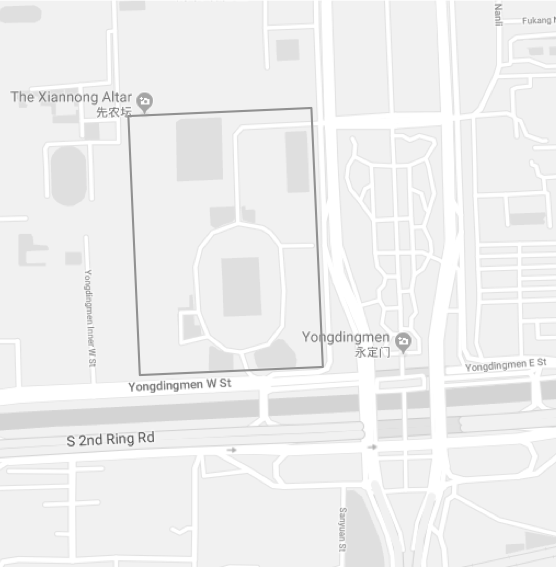
\includegraphics[width = \linewidth]{images/beijingXNT.png}
  \caption{Location of the Temple of the God of Agriculture Sports Technology Institute  (Source: Google Maps)}
  \label{fig:beijingXNT}
\end{figure}


\begin{figure}[htbp]
  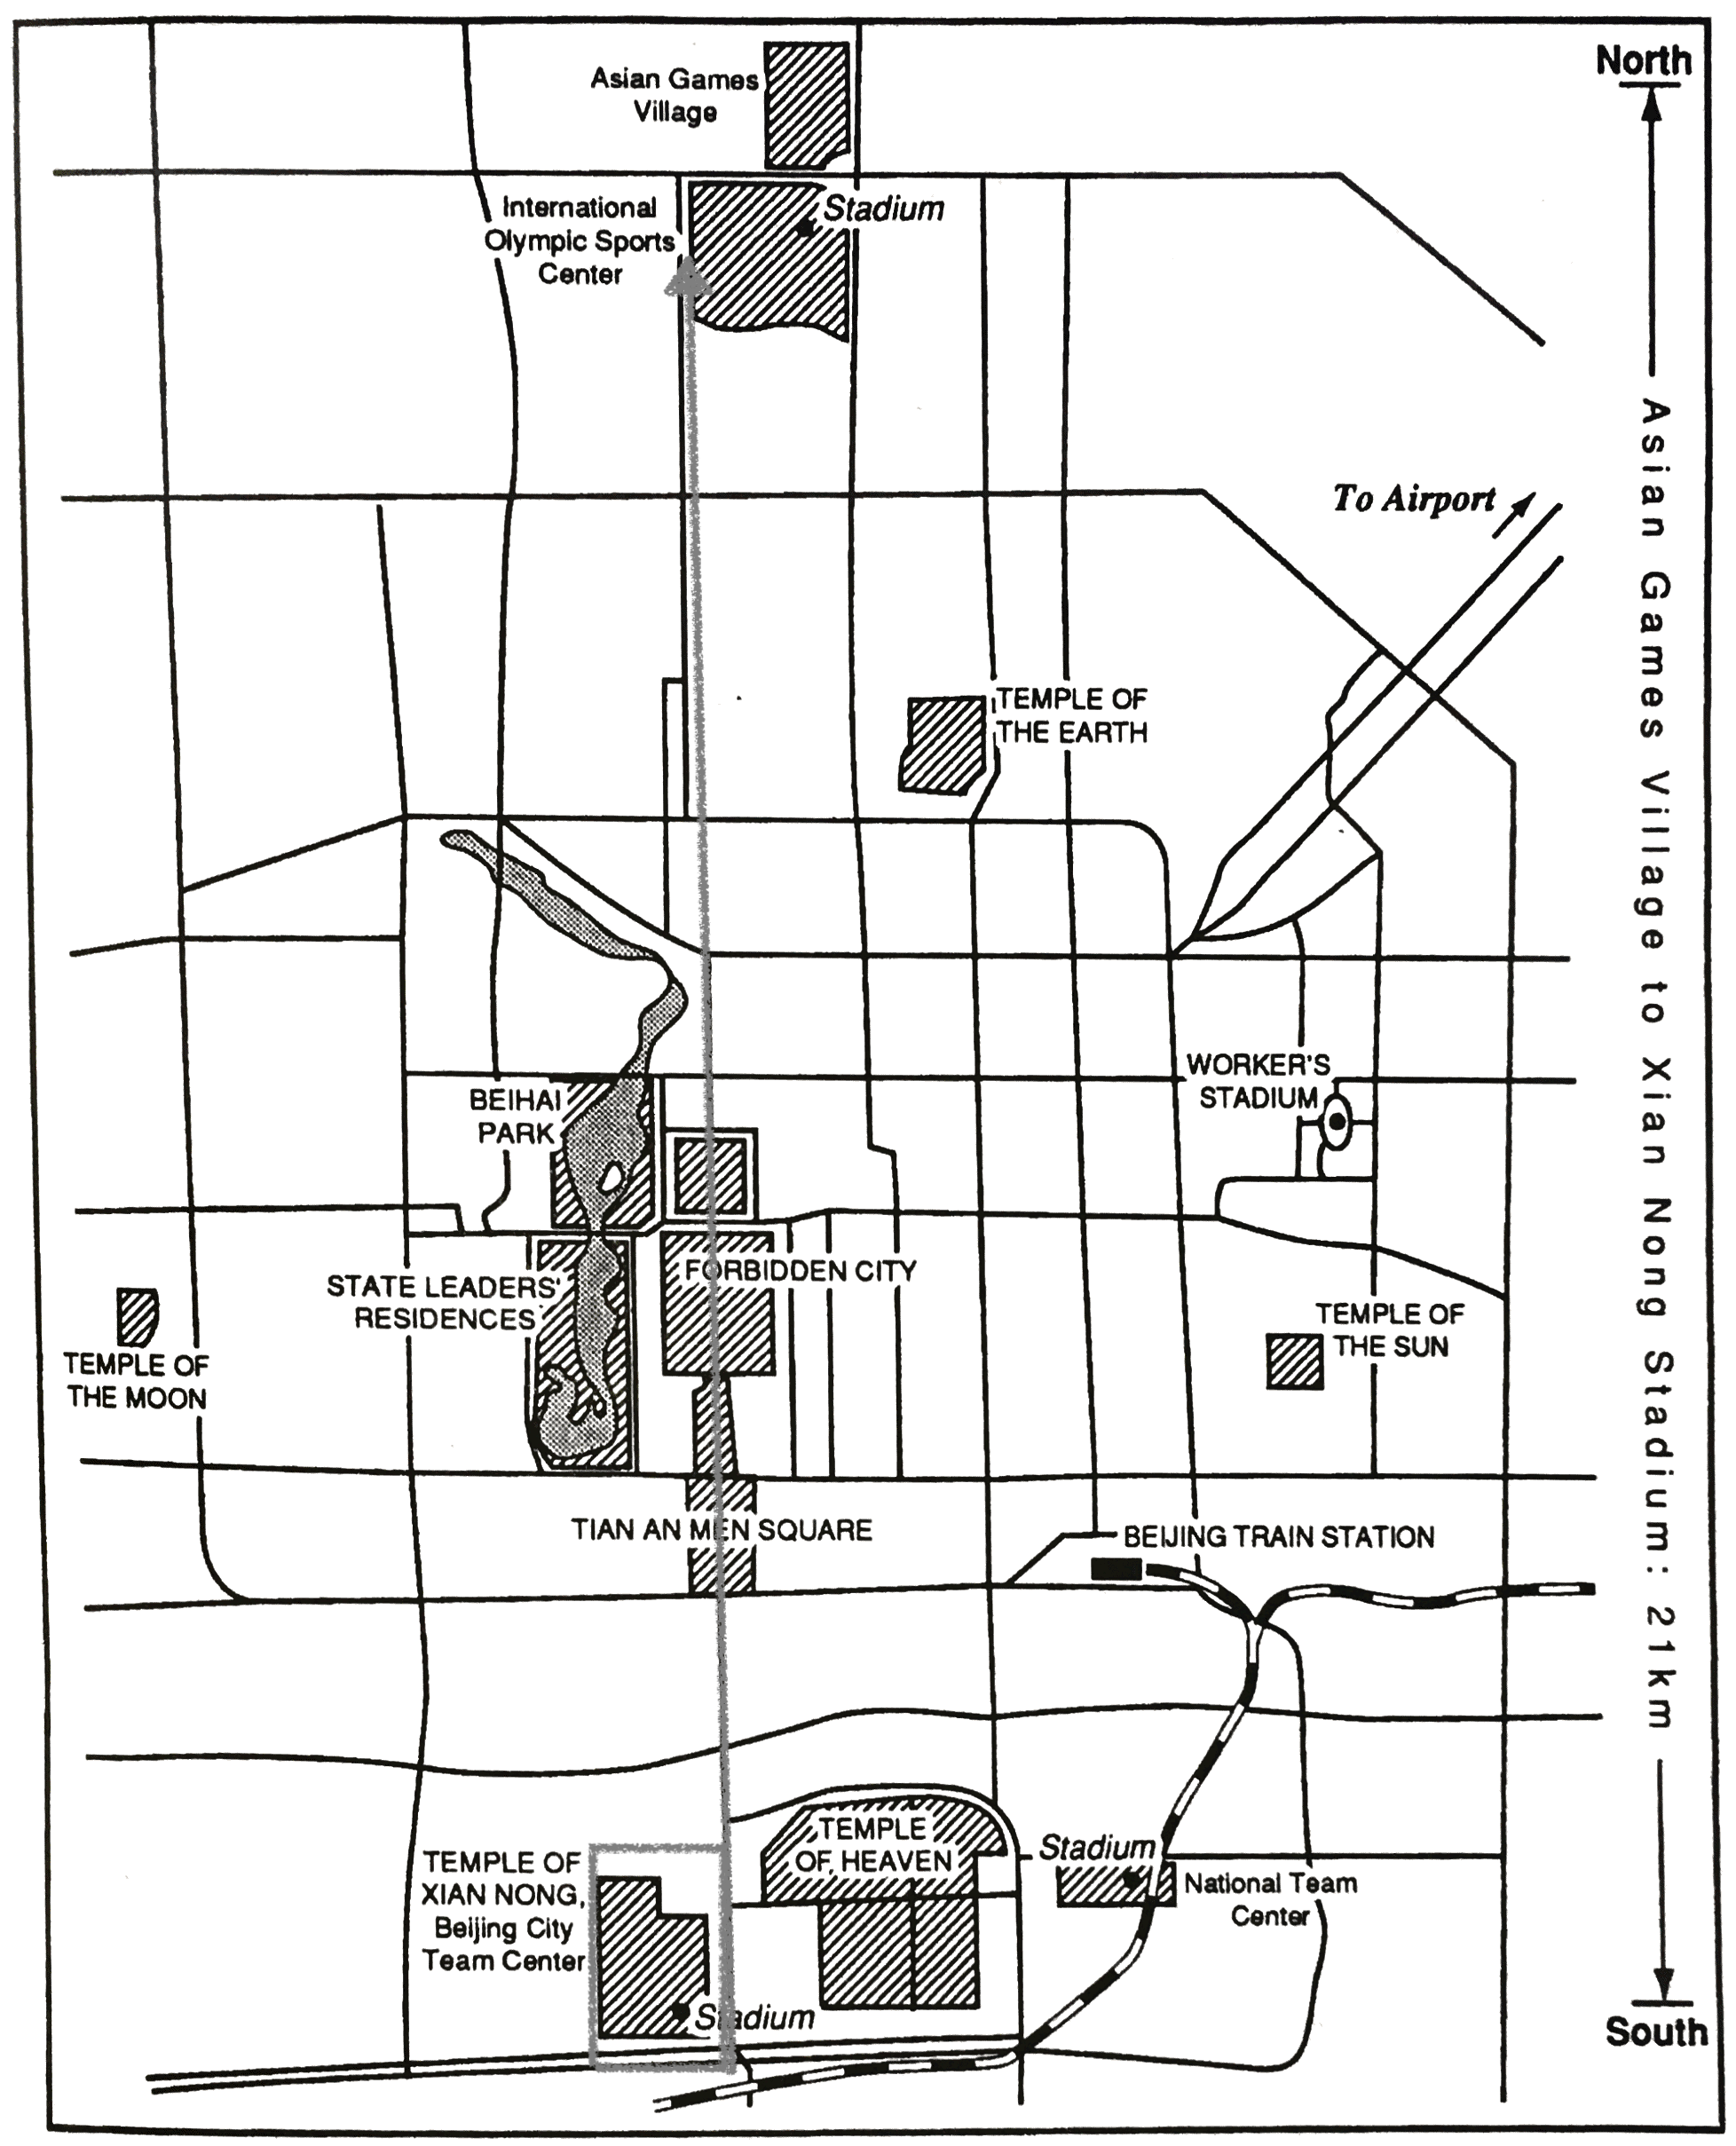
\includegraphics[width = \linewidth]{images/beijingTemplesXNT.png}
  \caption{Locations of former Qing dynasty temples (Brownell 2008)}
  \label{fig:beijingTemplesXNT}
\end{figure}


\section{Introduction}

A core assertion of this dissertation is that a scientific explanation of the cross-cultural prevalence of group exercise in human sociality must pay greater attention to the component mechanisms and system dynamics of joint action.  Existing experimental evidence linking group exercise and social cohesion is derived predominantly from laboratory experiments, in which essentialised components of group exercise---namely, behavioural synchrony and physiological exertion---are independently manipulated within dyads or small groups.  Results of these studies indicate that various forms of controlled and tightly coupled synchronised behaviour (from finger tapping to walking to rowing to talking) and certain intensities and durations of physical exertion (moderate to high intensity for minimum 30 minutes) are independently responsible for generating pro-social behaviour (Tarr2016), and may have some interaction effects (SOURCE). Existing evidnce sugggests that cognitive mechanisms associated with social interaction and neuropharmacological mechanisms associated with pain and reward mediate a relationship between group exercise and social bonding \citep{}. The activation of such mechanisms appear to  generate a psychophysiological environment---a ``social high''--- conducive to social affiliation and in-group cohesion \citep{Davis2015}.  Cultural group selection provides a theoretical explanation for the cross-cultural prevalence of group exercise in the contemporary and historical record \citep{Dunbar2010,Whitehouse2014a}.  In this dissertation, I argue that this ``social high'' account of group exercise relies heavily on laboratory studies that essentialise the components of group exercise, and as such lacks a sufficient understanding of the coordination dynamics of group exercise observable in real world settings.  Annecdote from highly skilled joint action practitioners, and emerging theory evidence from the social cognition of joint action supports the possibility that the proximate mechanisms of group exercise may require dynamic coordination of a certain \textit{quality} in order to generate pro-social behavioural outcomes.  The social high of group exercise may in some instances depend crucially on the ``click'' of coordination in joint action.

Sporting anecdote has for some time pointed to the importance of quality of coordination in processes of affiliation and team cohesion.  In the case of highly skilled practitioners in particular, the ecstasy of group activity appears to be contingent not on mere participation in joint activity, but on the perceived achievement of fine grained alignment of behaviour with co-participants.  The psychology of flow offers support for this dimension of reward associated with peak athletic performance \citep{Jackson1995}. Scientific knowledge of flow states, however, remains heavily restricted to individual level neurocognitive and psychological processes, and thus lacks insight into specific mechanisms and coordination dynamics of joint action.  Promisingly, a combination of 1) a recent paradigm-shift in cognitive science away from static input-output computational models of information processing towards ``active'' inferential models based on mechanisms of prediction and free-energy minimisation \citep{Friston2010,Clark2013}, and 2) empirical research programs dedicated to broadening the frame of analysis of social cognition to include interactions involving the affordances of distributed throughout the brain, body, and the social and physical environment \citep{Semin2008}, have begun to confirm elements of intuition and anecdote related to the phenomenon of ``team click.''  This dissertation offers a novel theoretical framework and a mixed-method step-wise empirical investigation into the relationship between coordination in joint action and social cohesion.

Evidence suggests that the perception of tacit understanding, team atmosphere, and general order in alignment of behaviours with co-participants (the dimensions of team click outlined in Chapter 2) could be due to the activity of a suite of cognitive mechanisms associated with 1) lower level sensory perception and movement regulation processes, 2) formulation of action plans in joint action, and 3) represention and communication of joint action goals \citep{Semin2008,Frith2008,Pesquita2017}.
%Evidence suggests that joint action specific processes bootstrap on lower-cognitive mechanisms associated with movement regulation.
Importantly, skilled practitioners in particular demonstrate a capacity to co-regulate movement in joint action such that joint action resembles an functional interpersonal synergy (SOURCE).  Functional interpersonal synergies are coordinative structures capable of reducing informational undertainty in a cognitive system ( - Noy2015? 2011). In this way, interpersonal synergies can be understood as extra-neural mechanism for minimising cognitive free energy in complex interactional environments (SOURCE). There is evidence to suggest that the formation and successful regulation of functional interpersonal synergies is underwritten by a regime of neuropharmacological reward \citep{}, suggesting a human capacity to discriminate on a spectrum of low to high quality coordination, and a psychophysiological preference for the latter end of the spectrum.  By examining in detail the phenomenon of team click in a joint action context involving highly skilled practitioners, this dissertation illumintes the way in which component mechanims and coordination dynamics of joint action typical of group exercise contexts may be relevant to processes of social bonding and group cohesion.

%The perceived click of joint action with co-participants in group exercise offers a way-in to quanitfying this coordination in real world settings.
% (repetition) In sum, it appears that in some instances, what is crucial to the social high of group exercise is not mere activation of mechanisms of behavioural synchrony and exertion, but the \textit{coordination} and \textit{quality} of the activation of these mechanisms.

A key insight overlooked by the existing social high account of group exercise and social cohesion, but revealed by the paradigm shift surrounding the social cognition of joint action, is the sensitivity of joint action (or any cognitive process for that matter) to informational affordances provided by various layers of ecological and cultural context.  The cognitive inputs to joint action in real world settings are rarely limited to essentialised componnents administered in laboratory paradigms. Cognitive processes relevant to joint action are known to be distributed throughout brains, bodies, and the physical environment of the ecological niche in which it is situated (SOURCE Ray2018 - multiple frames of reference). Indeed, the embarrasing fallacy of the experimental approach, now revealed in widespread attention to the ``reproducibility crisis'' in social science (SOURCE), is that even the controlled spaces and procedures of experimental studies are laden with unquantified cognitive affordances, often culturally specific, that contrain and enable quanitfiable outcomes (SOURCE).  I draw attention to this point not to denounce the usefulness or importance of the experimental approach to identifying generalisable mechanisms relevant to causal explanations of observable human behaviour; rather, I suggest that the experimental approach ought to be reevaluated in light of an emerging paradigm shift in cognition, in which the causal primacy of discrete cognitive mechanisms is challenged by the inherently distributed reality of cognition and the importance of coordination dynamics for its operation.

Discussed as part of the theoretical framework outlined in Chapter 2, shared cultural knowledge can act as a ``coordination smoother'' \citep{Vesper2017} for joint action, enhancing the effectiveness and efficiency of joint action between co-participants who share a similar informational framework.  In the predictive coding paradigm, cultural habits and frames of reference act as ``hyper-priors'' that set the macro-contextual coordinates for joint action\citep{Clark2013}.  Contextual affordances for joint action appear to be be dictated by processes operating at multiple conceptual levels---from the micro-level predictive processes associated with movement action and perception, to the macro-level predictive frames offered by specific cultural and contextual niches---interact in complex processes of reciprocal causation to shape joint action (SOURCE).  Conceptualisation of the causal complexity of cognitive processes relevant to joint action in this way echoes a broader reconceptualisation of the causal complexity associated with change on an evolutionary timescale, which recognises that human behavioural phenomena is the result of a number of biological, cognitive, and ecological mechanisms that interact via reciprocal feedback loops spanning varying scales of time and space \citep{Fuentes2015}.

The Role of Culture: CAT (Sperber2014, )
%Link joint action and social bonding to information tranfer and therefore cultural evolution:

The this theoretical approach to the social cognition of joint action (and human evolution more broadly) accords neatly with anthropology's long-standing concern for honouring the distinctiveness of cultural trajectories, and offers a space for reconciliation between anthropology and cognitive and evolutionary approaches to human behaviour \citep{Whitehouse2012}.  Prior to appropriate acknowledgement of the complexity of cognitive processes and psychological phenomena, researchers within the human cognitive, behavioural, and evolutionary sciences (for example, cultural and developmental psychology, see SOURCE) have been prone to overlooking local cultural specificity and causal complexity when seeking to generalise to the human species results of studies conducted with mainly Western subjects and methods \citep{Henrich2010d}.  Research agendas and the specific experimental designs to which they give rise are shaped by the historically and culturally contingent assumptions and priorities---predominantly of ‘‘WEIRD’’ (Western, Educated, Industrial, Rich, and Democratic) societies and experimental samples.  It is now clear that the complexity of observable behavioural phenomena can only be addressed by embracing a plurality of methodologies to systematically document variation within---and not simply between---cultural niches \citep{Fuentes2016}.  Anthropology is thus well placed to expand upon accounts of group exercise, via methods ranging from ethnographic exploration capable of uncovering novel dimensions of behaviour and generating testable hypotheses, to quantitative techniques---e.g., experimental and mathematical simulation paradigms---capable of testing hypotheses

In honour of the capacity of cultural and ecological trajectories to shape and direct observable behaviour in distinctive ways, the three empirical components of this dissertation are confined to one specific research setting---professional rugby in the People's Republic of China. Each study builds on the previous study in a step-wise manner, and as such the the cultural and ecological affordances associated with the group exercise context can be identified and held relatively constant.  In order to explore the validity of theoretical predictions (formulated in Chapter 2) in a real world group exercise setting,  I begin with an in-depth ethnographic study of the Beijing Men's Rugby Team.  I then refine my theoretical predictions based on the results of ethnographic analysis, and test these in an \textit{in-situ} survey study of a more representative sample of professional Chinese athletes before, during and after a National Championship Tournament.  These two studies provide the necessary grounding for a controlled field experiment designed to interrogate specific mechanisms hypothesised to underpin the phenomenology of team click and social bonding in joint action.  The empirical findings of this dissertation confirm 1) the relevance of component mechanisms and coordination dynamics of joint action to processes of social bonding and group cohesion, and 2) the importance of a diverse and coordinated methodological approach to measuring human behaviour---one that honours the contextual complexity of informational affordances in which cognitive processes are distributed and grounded.



In order to provide a sufficient contextual grounding for the three empirical studies that follow in this dissertation, in this Chapter I introduce 1) the parameters of joint action associated with rugby union, 2) important psychological and cultural factors relevant to social cognition of joint action in China, and 3) a history of physical activity and sport in China, from which rugby in China has emerged and in which it remains situated. I also outline the (unique) combination of qualifications that enabled me to conduct research in this specific context.  I conclude the chapter with an update to theoretical predictions of this dissertation in light of the specificities of the research context of rugby in China.

%In order to set the scene for the empirical studies of this dissertation, therefore, in this chapter I introduce the specific group exercise context of professional rugby in China.  I identify in the activity of rugby union and the cultural trajectory of China evidence for the social relevance of joint action, including evidence relating to the phenomenon of team click in both contexts.   I then outline the history of physical activity and sport in China from which my specific instance of rugby in China emanates.  I then outline of the (unique) combination of qualifications that enabled me to conduct research in this specific context.  I conclude the chapter with an update to theoretical predictions of this dissertation in light of the specificities of the research context of rugby in China.



\section{The Group Exercise Context: Rugby union in China}
The task of introducing the specific group exercise context of this dissertation requires a consideration of 1) the micro-level components and dynamics of joint action typical of rugby union (specifically rugby 7s), and 2) a description of the way in which these micro-level processes interact with, and are shaped by, the specific historical and cultural trajectory in which they are embedded---namely, sport in the People's Republic of China.  The experience of professional rugby players in China is nested within various layers of China's modern history, defined by projects of governance, state building and participation in the international community.  The cultural affordances recruited to facilitate these political and social activities---of which sport is central---emanate from a range of sources both foreign and indigenous to China, and have evolved as the result of China's modern history of confluence and antagonism with the world beyond its sovereign borders \citep{SOURCE}.  As such, while the prescribed rules of rugby union are legislated by an international governing body and therefore in theory consistent across the globe, the rugby played in China exhibits a particular style and quality that relates to the institutions, social norms, and culturally-shaped tendencies of action and perception specific to China. In this section, I note the relevant components of joint action typical in rugby contexts, and I outline the relevant layers of context in which this joint action is enmeshed, up to the present moment in China.

  \subsection{Rugby Union}

The parameters of joint action typical in rugby union make the sport highly suited to test the theories prescribed in Chapter 2, namely, the relevance of mechanisms and coordination dynamics of joint action to processes of social cohesion.  Rugby union entails high levels of both physiological exertion and socially-coordinated movement, and is anecdotally and colloquially associated with social bonding.  In this section, I introduce the specific history and dimensions of the group exercise context.

Rugby Union (hereafter rugby) is an interactional team sport played on a rectangular field (100m x 70m), by two teams, usually of 15 players, who physically contest possession of an egg-shaped ball that can be used to score points \citep{IRB2014}.  Descending from a variety of locally-specific folk-games played in pre-industrial England, all loosely grouped as ``football'', rugby developed within the elite public school system as a deliberate physical activity arbitrated by rules and regulations, before circulating through the arteries of England's colonial empire as a leisurely pastime—--a ``sport'' \citep{Dunning2005}.  In 1996, rugby became a professional sport and is played as such in Western Europe and in the Southern hemisphere. Rugby sevens---the specific focus of this dissertation---is a modified version of the conventional 15-a-side game involving teams of 7-a-side (rather than the conventional 15), and 14-minute games played in a Tournament structure over two or more days (rather than a one-off 80-minute match between two teams).  Rugby sevens has grown in popularity more recently, particularly since its introduction to the Olympics for the 2016 Games in Rio de Janeiro.  More so than the traditional version of the game, rugby sevens is played by countries all over the world, and attracts more balanced participation by men and women.

Rugby is a highly interactive and physiologically demanding sport in all forms and at all levels at which the game is currently played. Rugby requires players to participate in frequent bouts of intense activity at and above the aerobic threshold such as sprinting, physical collisions, tackles, and grappling, separated by short bouts of low intensity activity such as walking and jogging.  Rugby requires high levels of interdependence between team members due to the uncertainty and complexity of interactive coordination tasks.  At the elite level in particular, the physiological costs and complexity of joint action requirements of rugby are amplified.

Rugby, like many equivalent team sports in which a single ball (or similar object) is contested, such as basketball, association football, and ice hockey, is made up of a series of sub-phases involving attacking and defending sub-units \citep{Passos2011}. This structure of play requires athletes of these interactional team sports to perform and continually repeat similar joint actions with teammates.   The highest order of joint action in rugby sevens---the version of rugby most relevant to this dissertation---consists of 14 athletes (7 per team) who coordinate around the shared goal of completing a 14 minute game in which one team competes against the other team for victory. Lower-order goal-directed joint actions are nested within this overarching frame.  Depending on which team is in possession of the ball, players coordinate their movements around shared goals of attack or defence.  Completing the goals of attack and defence usually require coordination between sub-units of 2-4 athletes per team.  The goal of attacking subunits is to penetrate the defensive line or to at least advance towards the opposition's try line by securing possession at the ``breakdown'' (the contest for possession that occurs after a ball-carrier is tackled and brought to ground) in order to score points during a later sub-phase of attack.  The goal of the defensive subunit is to halt the ball-carrier and subsequently successfully contest possession of the ball at the breakdown.

There is very little direct empirical evidence specific to rugby union that can be used to substantiate a link between joint action and team click, and team click and social bonding.  Despite this, rugby is a sport heavily associated with the popular interpretation of ``social bonding,'' particularly in all-male social organisation common in the elite educational spaces of England and Commonwealth countries in which rugby originally developed \citep{Dunning2005,Richards2007,Collins2008}.\footnote{Recently, rugby union has been the site of much criticism due to the fact all-male social spaces cultivated by rugby appear to support and sustain hyper-masculine and hyper-normative behaviours, including gender-related violence \citep{Cosslett2014}.

``Rugby is a game for barbarians played by gentlemen,'' or so the saying goes.\footnote{The origins of this oft-cited Rugby adage is unclear.  The phrase is supposedly the adopted motto of the British Barbarians Football Club, established in 1890 \citep[34]{Dunning2005}.  The complete phrase reads ``Rugby is a game for barbarians played by gentlemen, football is a game for gentlemen played by barbarians.''  However, official club history cites its original motto as, ‘Rugby Football is a game for gentlemen in all classes, but for no bad sportsman in any class' \citep[vii]{Starmer-Smith1977}.  Some sources attribute the saying to British writer and poet Oscar Wilde (1854-1900) \citep{Fleenor2015}}. Different inflections on this adage have been reproduced by people in all parts of the world that rugby has reached (including China \cite{}), presumably as a way of linking the nature of rugby's physical requirements with social virtues of fair play, cooperation, and moral integrity. For example, the current slogan of World Rugby, the international governing body of rugby union, is ``Building character since 1886'' \citep{WorldRugby2017}, referring to the moral character that can be generated through participation in rugby.

  %P: Athletes are making a series of calculated but low probability bets -- such is the nature of competitive interactive team sports (Predictive coding paradigm).

  %P: finely tuned calibration of behaviours in environment of high uncertainty

  There is evidence to suggest that dynamic coupling occurs between dyads and sub-units of attack and defence\citep{Passos2011,Correia2014}.  Passos and colleagues \textcite{Passos2011} for example find that functional coupling tendencies emerge between attacking dyads and adapt to specificities of the task environment.  Correia and colleagues \textcite{Correia2014} show that coupling tendencies also emerge between co-actors of opposing teams in rugby union, for example, in a 1-on-1 attacker/defender sub-phase.  These results are confirmed in similar joint action contexts in other equivalent sports such as basketball and association football \citep{Duarte2013}. There is evidence to suggest that the establishment and maintenance of functional  interpersonal synergies in rugby joint action depend on an athlete's perception of affordances of the task-specific cognitive system made up of constraints including other athletes, the physical environment, and the rules of the game \citep{Passos2012}.

% P: Cognitive threshold for maintaining social bonds
  Dunbar \textcite{Dunbar1992} proposes that the ratio of human neocortex size to total brain volume imposes an upper cognitive limit on realtime coordination of behaviour of  4-5 individuals.  The group size of joint action sub-phases and sub-units in rugby sevens (2-4) fall within this upper limit, or just above the upper limit if attacking and defending subunits are grouped together (4-8).  Each team of 7 is complemented by a further 5 reserves to make up a total squad of 12 who compete in a tournament setting.  In addition, the size of squads that train together outside of tournaments can range anywhere from 16 to 28.
  These group sizes also exist within the cognitive limits for maintaining face-to-face intimate relationships, thought to be in the realm of 15-25 \citep{Dunbar1992,Dunbar2010}. These specific requirements of joint action in rugby sevens suggest that neurocognitive mechanisms responsible for tracking and monitoring coordination between co-actors and establishing interpersonal synergies between co actors will be particularly relevant \citep{Mogan2017}. (In addition to neuropharmacological mechanisms)


  In this case, the physiological demands, joint action complexity, and social-historical trajectory of rugby suggests that it is extremely suited to an investigation of the social bonding effects of joint action in group exercise.




  \subsection{Joint action, team click, and social bonding in China}

In addition to the parameters of joint action specific to rugby, the various cultural contexts in which rugby is played also have meaningful implications for behaviour observable in these contexts.  Sporting annecdote indicates that different teams from different places and times appear to play the same game in very different ways, often appearing to embody different ``styles'' of play (Taylor2010;SOURCES).  Shared cultural knowledge can serve to structure joint action scenarios in ways that help ``smooth'' coordination by providing pre-loaded expectations between co-participants \citep{Vesper2017}.  Theory from the predictive coding paradigm suggests that team click may not necessarily be limited to coordination of the most proximate joint action parameters of a particular group exercise setting such as rugby, but could rather be contingent on a snug fit between the specific demands of joint action and a whole assemblage of hierarchically ordered expectations and affordances pertaining to personal, cultural, and ecological trajectories \citep{Clark2013}.  Thus, a careful consideration of the culturally specific affordances relevant to coorindation of joint action and group membership in China is crucial to subsequent empirical analyses concerning professional rugby union in China. In the following section, I outline the cultural contours of the social cognition of joint action in contemporary China.

% Vollan2017 - cooperation under authoritarian conditions

%indigenous Chinese psychology
Understanding the cultural contours of the social cognition of joint action in China requires an engagement not only with contemporary findings from cross-cultural social psychology, but also with what social psychologist James Liu terms an ``indigenous Chinese psychology'' \citep{Liu2009}. For Liu, the construct of an Indigenous Chinese psychology is important for the purposes of deepening theorisations of observable social behaviour in China beyond the globally dominant Western modes of scientific knowledge production (including productions within human sciences such anthropology, psychology, and cognitive science).  A considerable amount of evidence has ammassed within cross-cultural and social psychology, for instance, which suggests that the existence of significant contrasts between samples of ``East Asian'' populations (predominantly undergraduates of Japanese, Chinese, and South Korean universities) and ``Western'' populations (predominantly undergraduates of North American and Western European universities) in domains of action and perception \citep{Peng1997,Nisbett2003}, self-construal \citep{Markus1991}, social group formation \citep{Yuki2003}, and institutional norms \citep{Liu2017}.  As Liu argues, however, broad brush generalisations based on this evidence alone run the risk of being frail to the obvious behavioural diversity between the East Asian nations, or indeed the undeniable variation that exists within each individual nation itself (for example, the internal variaiton in China between North and South; East and West \citep[see, for example,][]{Henrich2014}).

Instead, Liu and colleagues adopt a representational account of social identity \citep{Liu2005}, in which it is understood that socially shared representations of history are central to creating, maintaining, and changing psychological identity and patterns of social interaction. This approach allows for within- as well as between-group variation in observable psychological and cognitive patterns of social interaction in China.

  \subsection{Varying modes of Group Membership}

One area in which this application of Chinese indigenous psychology is particularly useful, is in the case of cultural variation in modes of group membership.  Anthropologists have for some time emphasised meaningful cultural variation in processes of group membership \citep{Strodtbeck1961,Kluckhohn1961,Mead1967,Fei1992}, and more recently cultural psychologists have sought to demonstrate this variation in experimental paradigms \citep{Markus1991,Nisbett2001}.
This research has produced a theoretical spectrum of group membership processes, the two poles of which can be described as ``categorical'' and ``relational'' \citep{Hofstede1980,Brewer2007}.  It appears that in the case of some cultural niches, traditionally ``Western'' cultures such as the USA, for example, the dominant core of self-definition is based on individual autonomy and separation from others.  By contrast, the self-concept of relational societies, many examples of which can be identified in East Asia (Japan, China, Korea, etc), is defined primarily based on social embeddedness and interdependence with others comprising their in-groups\citep{Leung2012}.  Both modes of group membership have been shown to shape attention, cognition, and behaviour \citep{Nisbett2003} and as such could have important implications for the task of identifying and measuring social bonding mechanisms of joint action.  Nisbett and colleages suggest that, as a general rule, East Asians subjects tend to be holistic, attending to the entire field and assigning causality to it, making relatively little use of categories and formal logic, and relying on ‘dialectical’ reasoning, whereas Westerners tend to be more analytic, paying attention primarily to the object and the categories to which it belongs and using rules, including formal logic, to understand its behavior’ \citep[291]{Nisbett2001}.

Variation in modes of group membership does not appear to be limited to broad ethnic or cultural groups, however. Indeed, the two predominant modes of group membership—--categorical and relational—--have been shown to vary across cultures (i.e. East Asian versus Western European or North American, see \citep{Markus1991,Nisbett2001,Yuki2003}, within groups (according to sex and personality differences \citep{Yuki2014}, and even within individuals (depending on contextual and situational primes, \citep{Lee2014,Wong2005}).  Although the durable persistence of cultural and linguistic institutions appear to be responsible for the prominence of one mode of membership over another, recently researchers have suggested that divergent modes of group membership—--categorical and relational—--may be mediated by context-specific socio-ecological factors such as the level of relational mobility in any given environment \citep{Oishi2010,Takagishi2014,Yuki2005}.

BUT: there is evidence that people of Chinese cultural origins are perfectly capable of behaving according to the tenets of social identity and self-categorization theory, even if this is not the default position

Hong et al (2000) shows that Chinese (albeit predominantly bilinguals) are perfectly capable of maintaining segmented, categorical forms of identity when the social and historical conditions make such an identity adaptive.

The representations of an indigenous Chinese psychology can be understood as the product of an ongoing interaction between 1) two milenia of institutional and cultural continuity (in the form of ancient Chinese dynastic civilisation), and a more recent history of interaction with with globally dominant Western modes of commerce, governance, knowledge production, nation-building, and international relations.






To fully comprehend an indigenous Chinese psychology and its role in shaping social interaction, a deep grounding in at least two dimensions of Chinese is necessary to extend and deepend.  First, Confucian philosophical tenets and their utilisation (in both dynastic and modern China) for the purposes of managing particularistic social relations as well as large scale state orchestrated political control, and 2) China's fraught and contested struggle to build a modern nation in the image of a prosperous and rejuvenated Chinese civilisation in the wake of 19th and 20th century imperial humiliations, is crucial in order to fully interpret, analyse, and predict observable patterns and dynamics of social behaviour \citep{Liu2009,Barme2009}.



Unsurprisingly, much of Anglo-American social psychology of the 20th Century is rooted in a categorical mode of representing and measuring group membership.  The canonical self-categorisation paradigm of social psychology \citep{Turner1987}, for example, requires that an individual make an identification between abstract categories of the self and the in-group or out-group. In this ``social identification'' paradigm, group membership is achieved when the perceived differences between the self and other in-group members are smaller than the differences between in-group and out-group members \citep{Yuki2014}.  In distinction to a categorical mode of group membership, relational group membership involves attention to maintaining and harmonising intragroup relationships, rather than engaging in intergroup categorical comparisons \citep{Yuki2003}.  In a relational mode of group membership, social identity is less a function of distance between abstract categories of self and in-group, and more a degree of commitment to cultivating a network of hierarchically structured---but more or less self-centred and self-enhancing---relationships \citep{Liu2009,Nisbett2003}.

Experimental evidence suggests that categorical group processes facilitate fast and effective identification with arbitrary minimal groups \citep{Diehl1990,VanBavel2014}, the arousal of intrapersonal cognitive dissonance between the self and experimentally constructed in-group \citep{Festinger1957, Stone2001}, higher levels of cooperation with categorically similar strangers in economic games \citep{Yuki2005,Yuki2003}, and greater attention to and memory recall \citep{Buchan2006,Ng2016}.  In cultural environments where relational processes of group membership are more prominent or salient, on the other hand, the inverse is usually observed. It has been noted, for instance, that minimal group experimental paradigms have had very little (if any) success in East Asian (particularly Japanese) contexts \citep[586]{Liu2009}.  Relational group processes, on the other hand, allow for the arousal of cognitive dissonance only when it is constructed interpersonally (as opposed to intrapersonally) between an individual and specific individuals to which that individual is connected by a meaningful social relationship \citep{Hoshino-Browne2005}.  Likewise, individuals with a predominantly relational group awareness are more willing to cooperate with and attend to strangers with whom they share relational rather than categorical ties \citep{Ng2016,Yuki2005}.

Evidence that higher levels of cooperation in Chinese subjects under an authoritarian leadership model, particularly when subjects self-report belief in the efficacy of authoritative over democratic leadership models.

The historical roots that have faciliatated the predominance of a relational mode of group membership run deep in China's history, rooted in Confucian \citep{Hwang1999}, folk-cultural axioms \citep{Wang2009}, agricultural modes of production \citep{Talhelm2014,Fei1992}, dynastic rule, and modern reinventions of these cultural forms by processes of the nation-state\citep{Liu2014}.

The metaphor of the family is particularly salient and pervasive in modern public representations.  On almost every scale of social organisation, from dyadic extra-kin friendships through to workplace interactions and macro-social organisations (cities, provinces, nation), the family and its relational priorities are consistently invoked to aid coordination and coerce participation in collection action.

Meanwhile, in the last 150 years of Chinese modern history, China's interaction with the outside world has also entailed the introduction of categorical group processes associated with the activities of the nation-state.  This combination of sources has led to a contemporary Chinese indigenous psychology in which a relational mode is predominant, and a categorical mode is contextually-activated, especially when categories such as ``China'' are threatened or challenged internationally \citep{Liu2009}.


of hierarchical relationalism (``guanxi''), dialectical and holistic reasoning, self cultivation, and ethical virtue ("human heartedness" or \textit{ren}) \citep{Hwang1987,Ho1998}, theoretical predictions concerning social interaction can become either overly abstract or seriously misleading.  In the case of this dissertation, a serious engagement with the cultural specificities of contemporary China---an indigenous Chinese psychology---is required in order to identify the contours of universally generalisable mechanisms that can explain a relationship between group exercise and social cohesion.


1. the ancient development of Chinese civilization as a singularly successful, multilingual enterprise, and
2. the recent development of Chinese nationalism in the context of its contemporary suffering and failures.
    * With the onslaught of Western imperialism over the last two centuries, traditional Chinese civilization collapsed, and traditional Chinese virtues came to be understood as flaws by leading Chinese intellectuals (see Levenson, 1959) and their political rulers.
    * The Confucian vision of state as ‘family and other particularistic social relations writ large’ became viewed as one of the reasons why Chinese people were unable to mobilize successful resistance to European and then Japanese invasion.
    * Generations of intellectual and political leaders sought to instill the ‘virtues’ of nationalism and patriotism to Chinese people as a means of mobilizing resistance to external aggression (Unger, 1996).

East asians are seen as relational, interdependent, dialectical rather than analytical reasoners, etc.

Self-focussed example in China,

Cross-cultural psychology has revealed interesting mean differences between Eastern and Western experimental samples with respect to self-construal and group membership, and similarities in terms of inter-group psychological processes associated predominantly with modern state building and the cultivation of national identity.

 in these contexts using only evidence from cultural and social psychology, would fail to sufficiently account for the richness of cultural affordances that enables and constrains observable behaviour.  Experimental evidence from cultural psychology suggests that, in contrast to ``Western'' subjects (predominantly English speaking North American and Western European University undergraduates), subjects from North East Asia (China, Korea, Japan) exhibit a dominant ``relational'' mode of social cognition,

  ---> the lack of ``team spirit'' and HXL's self-focussed team talk, for example, can lead you off the trail if you're working only with the surface deep findings from cultural psychology.

      Examination of indigenous psychology and its roots in a specific socio-historical trajectory reveals that this behaviour is in fact deeply pro-social.

  This mode of social cognition is identifiable in biases of action and perception (), social norms of self-construal and group formation (), and institutional design (Guanxi yang and legal system yin)

  and has its roots in the Chinese history of Confucian values

    Confucian philosophy of holism taken originally from Daoism
    Human heartedness and self-cultivation as the best way to participate in a social logic of hierarchical relationalism ()



  attention is directed to harmonisation of interpersonal relationships in hierarchical social organisation.



  Cultural Psych: relational self construal and group Membership
  Social Psych: inter-group identification theory (social identity theory)







%Joint action and social cohesion in China: 1) action/perception, 2) self-construal and social norms of group membership, 3) social institutions (guanxi and the state).
There is very little direct empirical evidence linking movement coordination and social bonding within the Chinese cultural context. There is, however, extensive indirect evidence from historical and contemporary psychological and anthropological literatures to suggest ways in which a relationship between joint action and social processes of group formation and cohesion is uniquely articulated in the Chinese context \citep{Weed2011}.  Taken together, this evidence suggests that China's specific trajectory uniquely enables and constrains social cognition in joint action contexts.  In this section, I outline evidence for the way in which an indigenous Chinese psychology, a construct generated through the product of socio-cultural institutions and a distinct historical trajectory---uniquely shapes social cognitive processes of action and perception, self-construal and group membership, and institutional norms \citep{Liu2009}.

1. Historical Evidence (Confucian philosophy etc)

%Confucianism:
% 1) Hierarchical relationalism
% 2) Holism
% 3) Human heartedness through self-cultivation


Contemporary China is a member of a cluster of North-East Asian nations (which includes Japan and Korea) that share elements of ethnic, geographical, and historical lineages.  One particular commonality is the fixation of applications of ``Confucianism'' to do domains of social interaction, ranging from intimate familial relationships, to extended kinship-like social networks, as well as relationships between the individual and the state (Liu2017).















  It is well documented that the most prominent cultural metaphor in Chinese social discourse is that of the family \citep{Maehr1980}, and that this metaphor structures many extra-kin social relationships between individuals, and between the individual and the state \citep{Gold2002}.  Traditionally, the father-son kinship relationship is utilised to naturalise the socially constructed relationship between lord and minister: ``Parents naturally love their children, and children naturally love and respect their parents, and they both know that they're stuck with one another no matter what...'' \citep[178]{Slingerland2014}. Likewise, the metaphor of family is often utilised to naturalise the notion of an extra-kin social group, for example a company or a sporting team \citep{Brownell2008}.  Whereas traditionally Western (Anglo-American) notions of group membership generally hinge upon a psychological representation of egalitarian equivalence between categories of self and group, the utilisation of the family metaphor for group processes relies on the individual identifying group membership through a participation in hierarchically structured (familial-like) \textit{relationships} \citep{Fei1992}.

  It is within these processes of extending familial metaphors to formal social relationships that Slingerland (2014) locates a key role for joint action. Inherent in the scaling up of familial relationships to extra-kin social relationships is the tension common to many collective action problems, that of vulnerability to free-riding and defection \citep{Cosmides2013,Gavrilets2015}.
  As Slingerland explains, the ``logic of civilised life makes us very keen to distinguish reliable cooperators from unreliable defectors...what we want then is a particular type of desirable...behaviour where there is absolutely no gap between action and motivation'' \citep[192]{Slingerland2014}. The paradoxical Chinese idiom of \textit{wei wuwei}, translated awkwardly into English as ``trying not to try'' or ``effortless action,'' is promoted in many ancient Chinese philosophical corpuses as a behavioural solution to conflicting incentives involved in coordination problems: effortlessness in performing socially desirable actions (virtues) communicates a level of mutual trust and commitment that is ``hard-to-fake.''  The phenomenology of effortless action is described at length in many of these corpuses, and is a key dimension of many traditional Chinese martial arts such as Taichi and Wushu \citep{Morris1998}.  Thus, although mass participation in Anglo-American competitive sports is only a recent phenomenon in China \citep{Brownell2008}, the social valorisation of certain types and styles of movement, particularly the phenomenology of flow in (joint) action appears to enjoy a long history in the resolution of social tensions inherent in collective action problems \citep{Slingerland2014}.





  More recently, research programs cultural psychology have generated evidence to suggest that cultural variation impacts on processes of action and perception \citep{Nisbett2003,Hoshino-Browne2005}, social learning \citep{Mesoudi2015}, and prosocial behaviour \citep{Yuki2005,Yuki2003}.  Research from cultural psychology relating to norms of self-construal can provide important insights into the way in which macro cultural processes interact with micro-dynamics of specific social interactions to structure and constrain cognitive processes implicated with joint action, team click, and social bonding.





1. Institutions:

2. Social Norms re group membership:

3. Action-Perception:


  \subsection{Joint action, team click, and social bonding in China}


  Historical evidence suggests that the dynamics of joint action in particular have the focus of ethical considerations, namely resolution of social tensions inherent in collective action problems \citep{Slingerland2014}.  It is well documented that the most prominent metaphor in Chinese cultural discourse is that of the family \citep{Maehr1980}, and that this metaphor structures many extra-kin social relationships between individuals, and between the individual and the state \citep{Gold2002}.  Traditionally, the father-son kinship relationship is utilised to naturalise the socially constructed relationship between lord and minister: ``Parents naturally love their children, and children naturally love and respect their parents, and they both know that they're stuck with one another no matter what...'' \citep[178]{Slingerland2014}. Likewise, the metaphor of family is often utilised to naturalise the notion of an extra-kin social group, for example a company or a sporting team \citep{Brownell2008}.
  It is important to emphasise that, whereas traditionally Western (Anglo-American) notions of group membership generally hinge upon a psychological representation of egalitarian equivalence between categories of self and group, the utilisation of the family metaphor for group processes relies on the individual identifying group membership through a participation in hierarchically structured (familial-like) \textit{relationships} \citep{Fei1992}.

  It is within these processes of extending familial metaphors to formal social relationships that Slingerland (2014) locates a key role for joint action. Inherent in the scaling up of familial relationships to extra-kin social relationships is the tension common to many collective action problems, that of vulnerability to free-riding and defection \citep{Cosmides2013,Gavrilets2015}.
  As Slingerland explains, the ``logic of civilised life makes us very keen to distinguish reliable cooperators from unreliable defectors...what we want then is a particular type of desirable...behaviour where there is absolutely no gap between action and motivation'' \citep[192]{Slingerland2014}. The paradoxical Chinese idiom of \textit{wei wuwei}, translated awkwardly into English as ``trying not to try'' or ``effortless action,'' is promoted in many ancient Chinese philosophical corpuses as a behavioural solution to conflicting incentives involved in coordination problems: effortlessness in performing socially desirable actions (virtues) communicates a level of mutual trust and commitment that is ``hard-to-fake.''  The phenomenology of effortless action is described at length in many of these corpuses, and is a key dimension of many traditional Chinese martial arts such as Taichi and Wushu \citep{Morris1998}.
  While mass participation in Anglo-American competitive sports is only a recent phenomenon in China \citep{Brownell2008}, the social valorisation of certain types and styles of movement, particularly the phenomenology of flow in (joint) action appears to enjoy a long history.









\section{Historical Context of rugby in China}

\subsection{Physical activity in Chinese modern history}
The history of Sport and exercise in China is in many fascinating ways emblematic of broader---often fraught and turbulent---processes associated with China's modernisation.  Beyond physical cultures indigenous to China, or practices imported much earlier in history from south Asian religious traditions (e.g. Buddhism and Hinduism), the emergence of Anglo-American interactional team sports and European calisthenics in China is entangled with a history of interaction, conflict, and embrace with foreign influence during the 19th, 20th, and 21st centuries.

  \subsubsection{Introduction, rejection, and embrace of sport and exercise in China 1842-1912}
By the beginning of the 19th century, China had established flourishing international trade relationships with Western empires.  Generally speaking, China traded in tea, silk, and porcelain, meeting high demand in emerging middle class households of newly industrialised nations of England, France, and Germany.  In return for these goods,   merchants from Western empires initially paid in silver, until it became clear that a trade imbalance was emerging between China and the West, owing to the fact that tea, silk, and porcelain where much more replenishable than silver \citep{Fay2005}.  Thus, by the late 19th century Western powers increasingly sought alternatives to silver, for which opium provided a much more replenishable (and addictive) solution.  By the mid-19th century, however, a series of conflicts arose between Qing dynasty rulers and the Western empires over the regulation and trade of opium, leading to the first Opium War (1939-1942).  The resulting Treaty of Nanking (1842) initiated a period of colonial occupation of China that drastically weakened the political power and legitimacy of the Qing Dynasty and increased the influence of foreign powers within China's major inland and port cities.

Increased foreign influence in China during this period brought with it the introduction of an array of ideas and practices to China's urban elite ruling classes, including novel physical cultures of dress, adornment, leisure, and exercise.  Increasingly popular at the time in Europe and North America was the belief that sport and exercise were important pedagogical tools in the development of physically and mentally strong subjects of post-Enlightenment modernisation \citep{Elias1986}.  This belief largely gelled with the values of a nationally (and internationally) motivated Chinese urban elite, and subsequently manifested in China in the promotion of Anglo-American competitive sports by North American Christian missionary organisations such as the YMCA (Young Men’s Christian Association), and the incorporation of calisthenics routines into military exercises \citep[240]{Morris2004}.  Such techniques were soon popularised within elite intellectual communities as pedagogical tools designed to foster an explicit link between the strength of the physical body and the strength of the Chinese nation \cites[32]{Morris2004}[49]{Brownell1995}.

The introduction of novel political ideas to China in the late 19th century involved importation \textit{en masse} of novel linguistic, cultural, and social categories and practices from the West and Meiji Japan (1868-1912) \citep{Liu1995}. \textit{Tiyu} (体育), the term in modern Chinese that most closely translates to sport, was one of many neologisms inherited from the Western social sciences via its Japanese translation.  Importantly, tiyu encompasses more than just the modern Anglo-American competitive sports (roughly translatable to ``yundong'' (运动) that the English word connotes.  Instead, the modern Chinese notion of sport refers to an entire culture and discipline of the body that is deeply intertwined with the political project of Chinese modernisation and advancement \citep{Morris2004}.\footnote{As Lydia Liu (1995: 58) points out, even the notion of “China” itself as a term linked to a national imaginary, only began to emerge as such through interaction with Western missionary discourses concerning ``China'' during the 2nd half of the 19th century.}

The two-character phrase \textit{tiyu} is a contraction of a longer four-character phrase \textit{shenti jiaoyu} (身体教育), a direct translation of Herbert Spencer’s notion of  ``a physical education'' that first appeared in Chinese reformist intellectual Yan Fu’s ``On Strength'' 1895 \citep[9-10]{Morris2004}.  Now naturalised within the modern Chinese vernacular, compound words such as the ``body'' (\textit{shenti} 身体) and ``education'' (\textit{jiaoyu} 教育), as well as other fundamental conceptual social categories such as ``society'' (\textit{shehui} 社会) and ``culture'' (\textit{wenhua} 文化) all first appeared in their modern form as an arsenal of translated neologisms made popular by Chinese intellectuals in the late 19th and early 20th century who were grappling with ways to transform a dynastic realm crippled by colonial occupation and feudal backwardness into a strong nation in a system of modern nations \citep{Pusey1983;Schwartz1964;Liu 1995;Huters2005}.   Convinced that the body, \textit{shenti}, was crucial to realising this transformation, intellectuals rigorously subscribed to the Spenserian ideal of a physical education, which combined with a moral and intellectual education, as a ``cultivation of the whole moral, intellectual, physical, and aesthetic self'' (\textit{dezhitimei quanmian fazhan} 德智体美全面发展) \citep[10]{Morris2004}.

%\subsubsection{The Boxer Rebellion}
Novel regimes of sport and exercise were not uniformly embraced in China during this period, however.  The most organised movement of anti-foreign, anti-colonial, and anti-Christian resistance during the period 1842-1912 came in the form of an army of Chinese subjects from rural areas of Shandong was known as the ``Militia United in Righteousness'' (\textit{yihetuan} 义和团).  The Militia trained in martial arts and meditation and explicitly rejected Western forms of physical culture such as sport and exercise \citep{Brownell2008}.  The Militia's first target in the ``Boxer'' Rebellion (1900-1901, members of the Militia were known in English as the ``Boxers,'' due to the fact that they had been practitioners of martial arts that included boxing) was the Horse Racing track in Beijing situated at the south gate of the Temple of God of Agriculture---a site that had become heavily associated with the activity and influence of foreign legions.

In a somewhat harsh twist of fate for the Militia, the influence of modern sport infiltrated Beijing's sacred sites even further in 1901, when the troops of the Eight-Nation Alliance (United Kingdom, The United States of America, Germany, Japan, Russia, Italy, and Austro-Hungary) arrived in Beijing to relieve the besieged international legions.  During this period, troops from the UK occupied the Temple of Heaven to the east of Yongding gate, while US troops occupied the Temple of Agriculture to the west \citep{Brownell2008}. Compared to many other open public spaces in Beijing, the flat, open spaces of Beijing's temple grounds were conducive to the playing of Western sports common in garrison life such as field hockey and association football.  Throughout the final years of the Qing Dynasty, the sporting activities organised within the grounds of the Temple of Heaven and Temple of Agriculture attracted the participation of troops from other legions, as well as western missionary organisations such as the YMCA, and local Chinese elites \citep{Steel1985}.


\subsubsection{Republican Era (1912-1949)}
The combination of a weakened dynastic regime and the influx and development of new political and social ideas among China's urban intellectual elite led eventually to the Chinese revolution in 1911, and the establishment of the Republic of China (ROC) in 1912 \citep{Mitter2008}. Sport in China began to develop among urban elite along two main strands—--``competitive sports'' (\textit{jingji tiyu} 竞技体育) and ``games and calisthenics'' (\textit{ticao} 体操).  Traditional Chinese martial arts also made a resurgence during this period.  Although initially delegitimised within the New Culture Movement as elements of feudal superstition, members of the National Essence Movement (\textit{guocui yundong} 国粹运动) reappropriated martial arts to by aligning these practices with rational modernist ideas about sport and the body, at a time when sport became more significant for the articulation of an emerging national identity in the face of imperial powers \citep[38]{Brownell1995}\citep[45]{Morris2004}.  A significant aspect of competitive sports was the public spectacle of the ``games meets'' (\textit{yundonghui} 运动会), in which the performance of emerging national and international political identities could take place.  As early as 1908, the Chinese sport community enshrined the Modern Olympic Games (\textit{Aolinpike yundonghui} 奥林匹克运动会) as the pinnacle of participation in an international community of nations, and as such, the quadrennial global ritual has since preoccupied a collective Chinese sporting consciousness, and a Chinese national consciousness more broadly (\citep{Burnett2009;Barme2009;Brownell2008;Morris2004;Xu2008}.

The most sourthern point of Beijing's sacred north-south continued to feature prominantly in the development of sport in the ROC.  In 1914, the YMCA organised the first ever multi-sport event within the walls of the Temple of Heaven in Beijing, which the ROC nationalist government later labelled the Second National Games (the label of the First National Games of the Republican era was retrospectively assigned to the ``First National Athletic Alliance of Regional Student Teams'' multi-sport event hosted by the YMCA in Nanjing in October 1910) \citep[441]{Li2015}. The active reappropriation of the sacred spaces of the Qing Dynasty through activities such as team sport, allowed the foreign legions to perceive their occupation of these sites as a demonstration of superiority over the Qing court, and facilitated the ROC's priority of displacing traditional reverence of the throne \citep{Hevia1990}.

Beijing lost its importance as the centre of state power when the ROC moved the capital to Nanjing between 1928-1948.  In 1937, however, after the space surrounding the Temple of Agriculture had been repurposed for a range of leisure and amusement activities (including sport), a large sports stadium was constructed on the land directly to the south east of the main altar.  With a capacity of 10,000 people and a dirt association football field in the middle, the Beiping Public Stadium (as it was originally named) was the second ever modern sports stadium to be built in the ROC---the first being built two years previously in Shanghai for the hosting of the National Games in 1935.  The grounds immediately surrounding the stadium subsequently became the site for the Beijing Municipal Elite Sport Training facility, the predecessor to the current Institute.


\subsubsection{Sport in the People's Republic of China (1949-1976)}
Sport was transformed and politicised in radical ways following the establishment of the People’s Republic of China (hereafter PRC) in 1949.  As a key member in the New Culture Movement and the May Fourth Student Revolution, CCP leader Mao Zedong was a proponent of the Spenserian logic of physical education.   When the CCP took power in 1949, the centralisation of the proletarian body and the propagation of an ideology of active body-cultivation was such that \textit{not} ``training the body (for China)'' was considered bourgeois and therefore anti-nationalist \citep[58]{Brownell1995}.  The body of the worker (\textit{gongren} 工人), peasant (\textit{nongren} 农), and soldier (\textit{bingyuan} 兵员), as well as the body of the athlete (\textit{yundongyuan} 运动员), were glorified for their ``capacity for manual labour'' (\textit{laodongli} 劳动力 )---the ideological foundation for the ``proletarian revolution'' (\textit{wuchanjieji dageming} 无产阶级革命) (Ge and G. 2005: 91).  The ``emancipation ''(\textit{fanshen} 翻身) and glorification of the physical, labouring body is particularly explicit in the propaganda posters of the early Mao era (Ge and G. 2005: 87) (see Figure ~\ref{fig:motherlandStrength}).

    \begin{figure}[htbp]
      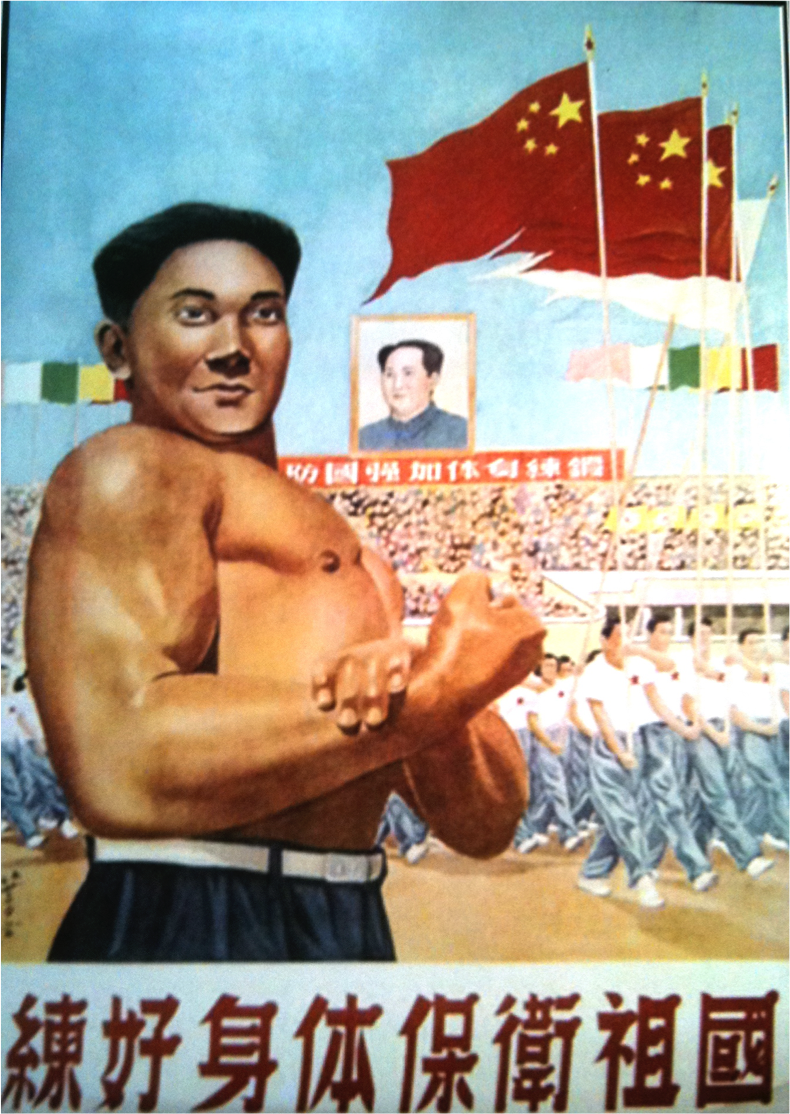
\includegraphics[width = \linewidth]{images/motherlandStrength.png}
      \caption{Strengthen Physique to Defend Motherland (1950)}
      \label{fig:motherlandStrength}
    \end{figure}


Along with many other facets of society after 1949, sport was institutionalised in line with Soviet bureaucratic models of governance.  In 1952 the ``State Sports (and Physical Culture) Commission'' (\textit{guojia tiyu yundon wieyuanhui} 国家体育运动委员会) (hereafter the Sports Commission) was established, which acted as the central State organ responsible for the administration of ``sport for the masses'' (\textit{qunzhong tiyu} 群众体育), ``physical culture education'' (\textit{tiyujiaoyu} 体育教育), as well as an elite competitive sport (\textit{jingji tiyu tixi} 竞技体育).  The competitive sport system was designed with the intention of creating a fast track for the development of world class athletic talent, in lieu of sports systems of western countries whose development pathways for athletes were more organically embedded within existing social and educational institutions. By creating model athletes capable of performing and advocating the healthy, egalitarian and militaristic body promoted by the Party, competitive sport was designed to kick-start more widespread engagement in ``sport for the masses'' and ``sport education''\citep[56]{Brownell1995}.

At the bottom of the hierarchical structure of the Sports Commission are local sports commissions (county, township and city), above which are the provincial and municipal sports commissions; and at the top is the National Sports Commission, located in Beijing \citep[59]{Brownell1995}.  The Sports Commission was responsible for all sports training centres and sports programs, of which there were many types.  On one extreme, the elite professional arm of the Sports Commission , a ``national (sport) system'' (\textit{juguo tizhi} 举国体制), which presides over all full-time professional sports teams (\textit{tigongdui} 体工队) that exist at national and provincial/municipal levels.  The main objective of this national system is to cultivate elite athletes to compete on a national and international level, in events such as the National Games (\textit{Quanguo yundonghui} 全国运动会), the Asian Games (\textit{Yazhou yundonghui} 亚洲运动会), and most importantly, the Olympic games (\textit{Aolinpike yundonghui} 奥林匹克运动会).  Due to an overwhelming Olympic-focus, all sports under the umbrella of professional arm of the Sports Commission are either Olympic sports, or Chinese martial arts (Guojia tiyu zongju 2009a).  Outside of this professional arm, elite sport programs are embedded within secondary and tertiary education institutions in a number of different ways, under the banner of the ``high school and university sport system'' (\textit{gaoxiaotizhi} 高校体制) (Guojia tiyu zongju 2009a).  At a high school level, elite sports programs are offered at ``extracurricular sports schools'' (\textit{yeyu tixiao} 业余体校), as well as regular high schools who focus on one or two sport programs in particular \citep[59]{Brownell1995}. At a tertiary level, a number of specialist sport colleges operate at national, provincial/municipal and local levels.

The reinstatement of Beijing as China's capital immediately following the establishment of the People's Republic of China in 1949, had immediate implications for the Institute situated at the Temple of God of Agriculture.  The existing stadium was enlarged to a capacity of nearly 30,000, and lights were added to enable hosting training and events at night.  The stadium was host to many important sporting and political events between the years of 1949 to 1976, including a number of International football matches attended by high profile CCP members, including Mao Zedong and Zhou Enlai (see Figure ~\ref{fig:maoXNT}).  Despite becoming heavily entwined with political processes of the PRC during 1949-1976, sport and its development was also severely hampered by many factors during this period.  On the one hand, the internal political, social, and economic chaos of The Great Leap Forward (1955-58) and the Cultural Revolution (1966-77) detracted from a focus on development of sporting infrastructure and sporting development.  On the other hand, PRC's exclusion from membership in the International Olympic Committee (IOC) and thus participation in the Olympic games, limited China's ability to participate in sporting events on the International stage.

\begin{figure}[htbp]
  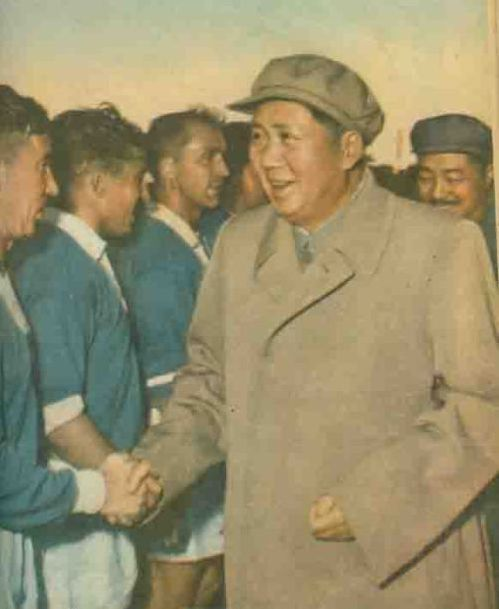
\includegraphics[width = \linewidth]{images/maoXNT.jgp}
  \caption{Mao Zedong congratulating members of the St Petersburg Zenit FC following a fixture against China in 1952}
  \label{fig:maoXNT}
\end{figure}


\subsubsection{Reform era tiyu (1976-2000)}
The death of Mao and the end of the Cultural Revolution in 1976 signalled the beginning of widespread social and economic transformations in China, in which the development of sport was heavily implicated.

Cultural Anthropologist Susan Brownell’s work, ``Training the Body for China'' (1995) was the first and most comprehensive attempt at an anthropology of sport in China. The research that forms the basis of Brownell's monograph was conducted during the mid 1980s at a time when China was only just beginning to interact politically and economically with an international community.


 In reference to the unprecedented success of the Chinese women’s volleyball team in the 1980s, including winning China's first ever gold medal in a team event at the LA Olympics in 1984, Brownell (1995: 86) explains how elite level sport functioned as a crucial symbolic practice for China in the process of ``rejoining the world.''  As a participant in the sports system as a student-athlete herself, Brownell draws on first-hand ethnographic experience of training and existing as subject to the state-administered ``microtechniques of power'' (citing \cite{Foucault1977}) designed to cultivate athletes in post-Mao China.


Brownell interrogates the role of the athlete in the perpetuation of a hyper-visible and generalisable moral order, cast in official terms as a ``socialist spiritual civilisation'' (\textit{jingshen wenming} 精神文明) (1995: 156).  Brownell explains that the position of the athlete in reform era China was one characterised by the tensions and shifts of an ever-transforming social terrain structured by contradictory forces of the state and the emerging logic of the market.

One of the most immediate transformations to effect the Chinese sports system after the death of Mao was the restoration of the University Entrance Examination (gaokao 高考, hereafter gaokao), following the end of the Cultural Revolution in 1976 \citep[198]{Brownell1995}.  School curricula were immediately redesigned around the gaokao, and as a result, schools quickly reduced emphases on sport programs as they were seen to draw student’s attention and energy away from academic study.  A situation thus emerged where the only option for prospective athletes was to attend a specialist sports boarding school in which a scholastic education was not emphasised or was abandoned all together in favour of intense physical training.

Success on an international stage in the early 1980s delayed public scrutiny of this widening gap between education and sport. The The PRC won a total of 32 medals at the 1984 Los Angeles Olympics---its first official appearance at the Olympics since it boycotted the games in 1952 due to a dispute with the Republic of China (now Chinese Taipei) over the use of ``China.''  Importantly, 15 of these 32 medals were gold, and this powerful display of strength on the international stage was an enormous moment for modern Chinese nationalism in the reform era \citep{Brownell2008}.

When China produced a much less impressive performance in the summer Seoul Olympics in 1988, winning only 5 gold medals (and a total of 28), latent public criticism of way in which reform era sport had become isolated from society readily surfaced and a ``crisis in Chinese sports'' was declared \citep[199]{Brownell1995}.  Amidst broader social anxieties concerning not only the alarming quantity of the Chinese population (renkou guoduo 人口过多问题), but also the problem of population \textit{quality} (renkou suzhi 人口素质问题), the athlete in China was problematised as lacking sufficient ``cultural quality'' (wenhua suzhi 文化素质) in accordance with his or her elevated social status as a ``representative'' (daibiao 代表) of the Chinese nation on an ever-expanding international stage (General Administration of Sport 2009a; Brownell 1995: 95).

In response to this public sentiment, in 1988 former army general Wu Shaozu (伍绍祖) was appointed head of national sports commission and tasked with implementing reform measures that would help the ``societization'' of the Chinese sport system. In 1989, for example, the Sports Commission adopted a policy modelled on the US college sports system, of ``combining sport and education'' (tijiao jiehe 体教结合).  In an attempt to move away from a reliance on sport boarding schools and full-time sports training centres for the development of athletic talent, ``high level tiyu programs'' (gaoji tiyu xiangmu 高级体育项目) were embedded within existing stand alone high schools and universities so as to ensure the ``all-round development''(quanmian fazhan 全面发展) of the athlete \citep[203]{Brownell1995}.  As part of an emphasis on a broader range of sports and their perceived potential to facilitate community engagement, international relations, as well as commercial opportunities, various sports programs, including many non-Olympic sports such as rugby, were inducted into the Chinese sports system for the first time\citep[70]{Knuttgen1990}.  Above all, the  democratisation of sports programs to include non-Olympic sports was driven by a persistent faith---built-in to the logic of ``physical culture'' form its inception int China---in the ability of sport to produce citizens of a certain \textit{quality} \citep[7]{Woronov2003}.

Reform measures continued into the mid 1990s. In an attempt to reduce the monopolisation of power and resources in the sports system, in 1993 Wu Shaozu broke up the six major sporting bodies of the Sports Commission into 23 sports management centres, with the ultimate goal of placing every sport under the management of an independent sporting association. In 1994 the first professional Chinese Football League was established, followed soon after by the professional Chinese Basketball League in 1995. In 1998, the Sports Commission rebranded as the General Administration of Sport (hereafter GAS) to accord with this direction of institutional reform.  But, one year earlier in 1997, powers above decided that Beijing would bid for the 2008 Olympics, and as such a subtle shift in focus occurred in Chinese sport that altered the course of reform.  Indeed, once the bid for the Olympics was announced as successful in 2001, sport reform ground to a halt as priority shifted to winning as many gold medals as possible \citep{News2017}.  Wu Shaozu left GAS in 2000, and his two successors Yuan Weimin (袁伟民, 2000-2004) Liu Peng (刘鹏, 2004-2016) did not actively return to the project of reform, continuing to invest in Olympic performance.  Even though many sports had since established independent associations, these associations had to be directly affiliated with one of the 23 GAS has 23 sport management centres. Rugby, for example, was affiliated with the ``Management Centre for Small Ball Sports'' (\textit{xiaoqiu guanli zhongxin} 小球管理中心),which was also home to sports such as golf and ten-pin bowling.

\subsection{Beijing Olympics and the lost decade of sport reform (2001-2012)}
    The lost decade:
    The structure of the sports system exists today largely unchanged, although its name changed in 1998 to “The General Administration of Sport in China” (国家体育总局 Guojia tiyu zongju) (hereafter the Sports Administration).
    Sport system became a space for scandal and corruption:

    Public discontent concerning the persistence of China's narrow performance-focussed sports system was palpable throughout the 2000s.

    CORRUPTION and SCANDAL:
    marred by controversy:
    corruption, match fixing etc
    Doping reports

    Yet, much like Groundhog Day, as was the case in the 1980s, these murmurings remained sufficiently muffled in public discourse by the strong performances of Chinese Olympic athlete delegations in Sydney 2000 (28 gold, 58 total) and Athens 2004 (32 gold, 63 total). The choreography of Chinese sporting might on the world stage reached its pinnacle when Beijing hosted the 2008 Olympics, with the Chinese athlete delegation winning 48 gold medals in a total haul of 100 medals.

    ``Low investment in public team sport, and deteriorating public health, contributed to lack of public participation, and the industry’s low value'' (Wang Qi). CBA and CFA have suffered years of losses, not to mention table tennis and volleyball”

    Many management centres have swelled into sovereign entities.

    Power and money were concentrated in one pair of hands -vulnerable to corruption.  sports centres have moved away from We’s original reform goal, and become a hindrance to development of sports industry.

\subsection{Xi Jinping Era sport reform and Beijing 2022 (2013 - present)}

    XI ERA REFORM:

    Beijing 2022

    Football:
    Sport in 2013 announced as domestic consumption

    Yao Ming

    Table Tennis Coach dismissed.

    Late 2016:  GZW blindisded sports centre managements, calling them monopolies and saying too much power rests in the hands of their chiefs.


    BZB:



  \subsection{The history of rugby union in China}



    \subsection{Rugby Union in China (1992-2009)}
Although reportedly existing in China within colonial and expatriate circles for more than a century (Reason and Carwyn 1979: 210; HKRFU 2009), and as a modified military exercise as early as the 1930s \citep[135]{Morris2004}, rugby was a late entrant into the Chinese sport system, established as a ``high level sport program'' in 1990.  The advent of rugby in China can thus be understood in terms of the processes of sport ``democratisation'' explained above.  The introduction of rugby into China was initiated originally at CAU by professor Shi Zhengsheng (施振声) who was introduced to rugby by his
supervising professor while completing vocational studies at Azabu University in Japan 1987-1989.  Following Shi’s return to CAU, an exchange relationship was set up between the two universities, and throughout 1990, coaches and referees from Azabu University came to CAU to help set up the necessary infrastructure required for a rugby program.  On the 12th December 1990, China’s first rugby union team was created.  The program was originally made up of existing CAU students who expressed interest in the novel activity, but by its second year, the program earned status as a “high level tiyu program” and was subsequently advertised to student-athletes across the country (Xu 2010: 2).  Between 1990 and 2010, rugby programs based on this original CAU model were established within over 30 regular universities and specialist sports colleges in cities throughout China.  There are also a number of social rugby clubs (\textit{julebu} 俱乐部), organisations completely independent of the state sports system, in major cities with high expat populations (Shanghai, Beijing, Chengdu, Qingdao).

The Chinese Rugby Football Association (CRFA) was established in 1997. Both the men and women’s national teams, made up of players predominantly from CAU, but also from other well-established programs based at the Shanghai Sports University, Shenyang Sports College, and the People’s Liberation Army Sports College. China consistently competes against other nations in the Asia Pacific region (most notably in the Asian Games and the East Asian Games), and are also occasionally involved in top-tier international tournaments such as the International Hong Kong Sevens.

Before rugby became a professional sport in 2010, it had existed as a non-professional university sport for 20 years.  First established in 1990 at CAU, Beijing, rugby was and still is part of a large collection of ``cold-gate'' sports (\textit{lengmen xiangmu}, a term that refers to a profession, trade or branch of learning that receives little attention) in China, with a relatively small participation base compared to other interactive team sports like basketball or football.  While football and basketball have matured as standalone enterprises with supporting market-based consumer industries, most other sports in China (i.e., all other Olympic events, including rugby) exist primarily due to the support of the enormous state-sponsored sport system.  Whereas the commercial basketball and football industries might offer a small percentage of prospective athletes incentives of fame and fortune, the benefits of a state-sponsored sports programs like rugby are more modest.  Chinese youth either gravitate or are ushered by their parents towards sporting careers primarily due to potential life-course opportunities such as access to tertiary education and post-athletic career employment (in the government sports system).  The extent to which an athlete is able to maximise these potential benefits depends on the strength of an athlete's results (\textit{chengji}).

In Olympic sports, the most important measure of a province's success in state-sponsored sporting terms is the National Games, a quadrennial multi-sport event hosted on rotation by provincial capital cities \citep{Hong2002}.  The amount of funding a province and its provincial sporting institutes and programs receive is decided to a large extent by results at the national games.

However, due to the persistent Olympic focus of the Soviet-modelled Chinese competitive professional sports system (\textit{juguo tizhi}), rugby's recently acquired Olympic status means that it is one of 33 sports featured in the all important quadrennial National Games.  Ten of China's collection of 32 provinces and municipalities that participate in the National Games have full time men's and women's rugby programs.


\subsection{Rugby in China 2010 - Present}

When rugby union was inducted into the state sponsored sports system in 2010, a few Chinese provinces in particular identified a potential opportunity to achieve a beneficial National Games result by heavily investing in this debutant sport.  Beijing's Temple of Agriculture Sports Institute managed to attract a large amount of China's existing rugby talent—---including the unofficially touted ``Emperor'' (Boss) (\citep{huangdi}) of Chinese rugby, national coach Zheng Hongjun—--from where they were previously based at the Chinese Agricultural University, Beijing.  Meanwhile, Shandong province—--a powerhouse in other provincial sports--—succeeded in attracting the majority of the remaining talent, by token of the fact that a large majority of rugby players in China at the time (indeed, a large proportion of athletes more generally) were of Shandong origin.  Importantly, this talent included the Emperor's student come rival coach Lu Xiaohui.  Besides Beijing and Shandong, Jiangsu and Anhui province were strong contenders for the women's gold medal, while the People's Liberation Army (PLA) and Hong Kong in particular were strong contenders for top spot in the men's competition.

Beijing's results leading into the 2013 national games were strongest overall across the men's and women's teams, however the Hong Kong men's and women's teams had only occasionally participated in these tournaments.  In the semi-finals of the National Games, the Beijing men came up against Hong Kong, while the Shandong men played off against the PLA.  Beijing lost to their stronger and more favoured opponents, whereas Shandong beat the PLA.  Meanwhile in the women's league, both Beijing and Shandong advanced to the final.  The stage was set: Beijing, the favourites led by the reigning Emperor of Chinese rugby, would face Shandong, the underdogs lead by the Emperor's cunning apprentice.

The men's final was played first, and in somewhat of an upset, Shandong edged out Hong Kong to win the gold medal by one try.  In the women's final, scores were level until early in the 2nd half when Shandong went ahead by two tries to nil.  At that point, the Beijing women's team, under instruction from their coach Zheng Hongjun, suddenly stopped playing.  After being asked by the referee and match officials to continue, the Beijing women stood firm and refused to play on, forming a huddle on their side of half-way in the middle of the field. Shandong had no choice but to continue to play out the rest of the 2nd half, running in try after try, until the final score at full time was a farcical 71-0.  Shandong was declared victorious, while Beijing called foul play, claiming that the referee had been unfairly adjudicating the match in Shandong's favour.  The details and dramas of this now well-known story in China's sporting history (known as ``Match-striking-gate'') require more detailed development in a format that exists beyond the scope of this particular study. I introduce the story here in order to highlight its implications for my ethnographic research.

The Beijing women's rugby team was the first Beijing team in the 48-year history of the National Games not to receive the ``medal for civilised spirit''  (awarded by the Beijing Mayor to all Beijing representatives in the National Games) (SOURCE).  All rugby coaches and many senior athletes of the 2013 National Games campaign have since left the Temple of Agriculture: either retiring or moving to other provinces.  The rugby program was all but abandoned in 2014, and finally at the end of 2014 the men's program was resurrected by the appointment of a new head coach Zhu Peihou (a former Agricultural University Coach) and assistant Coach Shiyan.  The women's program was only formally re-established at the end of 2015, with the appointment of former Beijing women's rugby representative athlete Ma Jiale as head coach, and former Beijing men's rugby representative athlete Wang Chongyi as assistant coach.  Rugby is still part of the institute, but is no longer centre stage, and is a shadow of its former glory.  It was in this context that I entered the institute and conducted ethnographic research.

The second implication of this incident is what it says about the ethics of group membership in China.  This is not the first match-striking incident of Chinese sport. In fact, match-striking features periodically throughout recent Chinese sporting history.  In July 2015 Chinese ping pong athlete Zhang Weike failed to turn up to the 9th Round of the ping pong league because in protest at his club's refusal to sign a competition bonus agreement with him for that particular round of competition. The club were holding off signing the agreement because due to Zhang's recent poor form.  In 2004, Beijing Moderns Football Team famously stopped playing mid game against Shenyang Jinde Football Team due to objections with the referee's decisions. It was later revealed in an extensive expose of Chinese football in 2009 that the referee had in fact been bribed to fix the match (along with many other matches during that period), and this incident and many other like it were linked to the control of professional football in China by mafia-run betting rings.

The relevance of this incident to the present study is the fact that match-striking—--a strategy that appears to publicly disregard the sanctity of ``sporting contest''---exists as a viable strategy in the Chinese sporting world. That this option and others make up the behavioural arsenal of athletes, coaches, and officials in competitive sport in China is first an indication that sport in China suffers from a general lack of trust in the institutions that supposedly stand for values of fair play, sportsmanship, and the sporting contest; values often celebrated in Western democracies to be the foundational pillars of sport and worthy of fierce deontological defence in and of themselves\citep{Morris2004,Gold2002,Yuki2005}.

There have been various concerted attempts throughout China's modern history to instil the importance of ``fair play'' in Chinese sport \citep{Morris2004,Brownell1995,Brownell2008}, and yet, however intensely politicians, sports officials, coaches, and athletes emphasise in official public rhetoric the importance of such categorical ideals in sport, it is also clear that the behaviour of these very same agents is often heavily determined by networks of power (\textit{quanli}) and interest (\textit{liyi}) that function externally to official institutions and threaten the exact values that are publicly promoted.



\section{Qualifications and positionality of the researcher}

  Before arriving in Beijing in 2015 to begin my doctoral research, the last time I was in China was two years earlier in 2013, when I spent eight months coaching the Chinese men's youth rugby 7s team in the lead up to the Nanjing Asian Youth Olympics.  Before that, I had spent one year studying on Exchange at Beijing University in 2008, and another year before that on an intensive Chinese language course at Liaoning University, Shenyang, in 2006---my first trip to China.  Rugby featured heavily in both instances.  In 2006, an Australian classmate and friend Ed had caught wind of the fact that there was a rugby program down the road from Liaoning University at the Shenyang Sports College (SSC).  Despite the fact that we had both been diligently attending class and courageously deploying our elementary Chinese to order food at restaurants and befriend local taxi drivers, Ed and I were, nonetheless, three months into our intensive language exchange and feeling that our Chinese skills were floundering.  We suspected that this was in large part due to the fact that we had met very few local Chinese people our age.  So one afternoon we rode our bikes over to the Shenyang Sports College in time for the rugby team's afternoon training session.  Less than six months later, we were boarding an overnight train from Shenyang to Shanghai with the SSC rugby team to compete in the annual Shanghai Rugby 7s Tournament.  We had become closely integrated into the community of rugby athletes at SSC, due in part to the common language of rugby that we all shared, and perhaps mostly due to the overwhelming hospitality of the SSC athletes and coaches.  The decision to find the rugby team may have also helped us improve our Chinese. Ed and I were the only two in our cohort to finish the year in Shenyang with a Level 6 in the Chinese Proficiency Exam, which qualified us to study alongside Chinese local students at an undergraduate level.

  Buoyed by this experience with the SSC rugby team in 2006, I followed a similar template two years later when I arrived at Beijing University on exchange from Sydney University to study sociology at Beijing University.  I had just finished working at the 2008 Beijing Olympics. At that time in Beijing, the only Chinese rugby program was based at the Chinese Agricultural University, a forty minute cycle north of Beijing University.  It was during my time training and generally ``hanging out'' at CAU that I met and developed a strong friendship with Kai, who was at the time playing for CAU and China, while also finishing a Master's degree in Labour Law.  I also met and developed relationships with many rugby players, coaches, and general fans of the Beijing rugby community.  The CAU rugby program was the strongest in the country: CAU consistently outperformed its rivals at the time (Shanghai Sports Institute, the People's Liberation Army, and SSC) and it was awarded with the responsibility of hosting the Chinese national team.  When the International Olympic Committee announced in late 2009 that rugby would be played in the 2016 Rio De Janeiro Olympics, it was subsequently decided in 2010 that rugby would be inducted into the the state sponsored sports system and played in the next Chinese National Games in 2013.  Following this announcement, many of CAU's athletes and coaches dispersed to various professional provincial rugby programs, the main ones being Beijing and Shandong.

  Between 2009 and 2013 I returned to Australia to finish my undergraduate degree, during which time my own rugby career also rapidly developed.  After a successful season in the Sydney premiership competition in 2009, I was selected to play for the Australian Rugby Sevens team. I represented Australia in Sevens from 2009 through to the end of 2012.  In 2013, during the 9 month gap between my Australian rugby contract ending and the start of my graduate studies at Oxford University, I returned to China to coach the Chinese Youth Men's 7s program in their lead-up to the 2013 Nanjing Asian Youth Olympics.  Along with a small team of Chinese coaches and management, I coached a core group of roughly 25 athletes aged between 15 and 18 years old. Our athletes trained 6 days a week for approximately 6 months, with only occasional breaks for National holidays, or for athletes to return to their home provinces to complete compulsory exams.  The program was based predominantly in Anhui province, and we travelled from Anhui to other provinces further afield to find suitable practice opportunities against provincial programs.  Soon after the completion of the Asian Youth Olympics in Nanjing in 2013, the Chinese National Games were held in Shenyang. Rugby was played---for the first time in National Games history---with dramatic consequences.


\subsubsection{Positionality of researcher}
%China,
%rugby intuitions and expertise,
%performance to the western observer





\section{Study Predictions}

\subsection{Social cognition of joint action among professional rugby players in China }


(What to expect)
